% !TEX root = ../beamer.tex

\begin{frame}[fragile, plain]
	\plainnumber
	\frametitle{Workflow Specification}
	
	\begin{minipage}{0.45\textwidth}
	    		        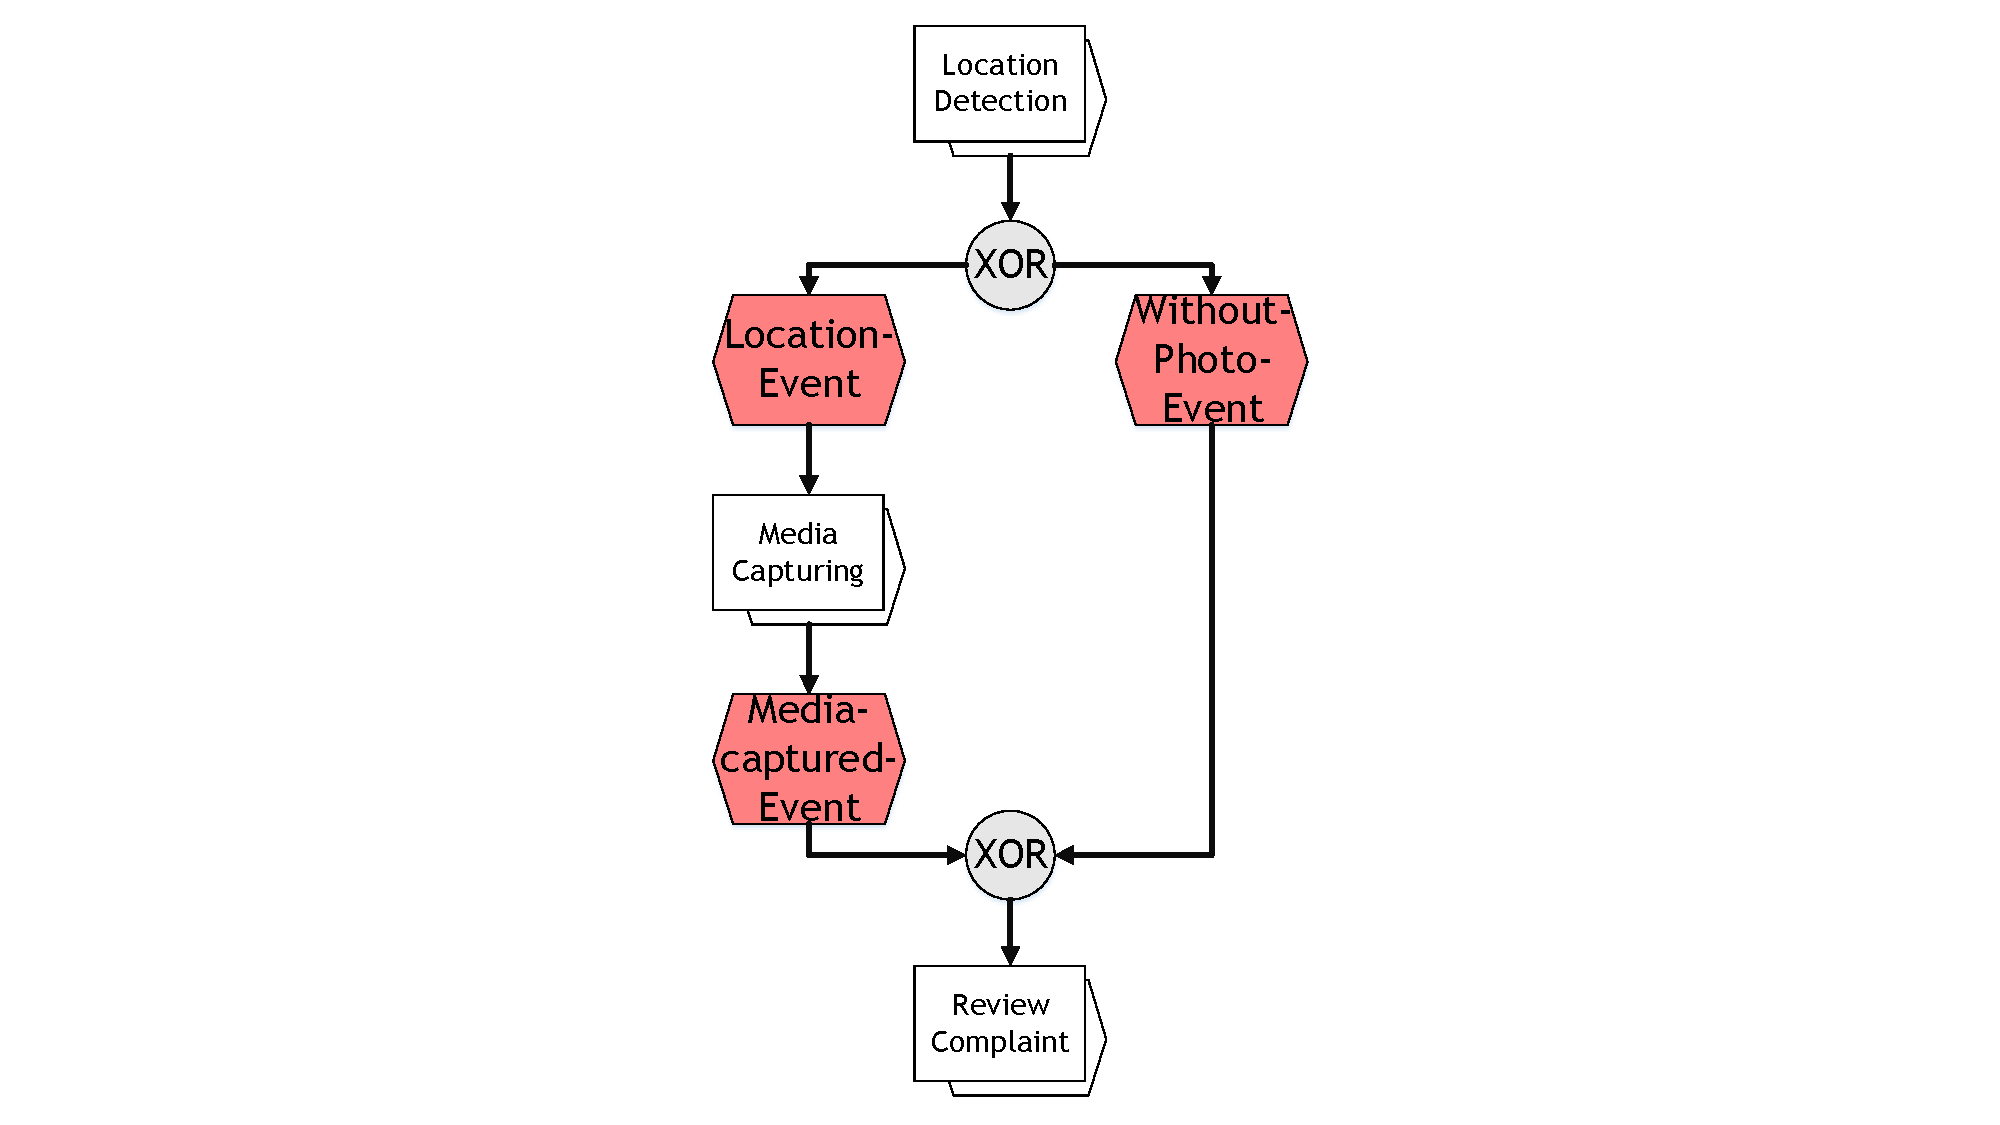
\includegraphics[height = 7cm, trim = 10cm 0cm 10cm 0cm, clip = true]{images/WorkflowSpecification.pdf}	  
	\end{minipage}\hfill
	\begin{minipage}{0.5\textwidth}
\begin{lstlisting}
WorkflowElement LocationDetection
  fires LocationEvent {
    start Mediacapturing
  }
  fires WithoutPhotoEvent {
    start ReviewComplaint
  }

WorkflowElement MediaCapturing
  fires MediacapturedEvent {
    start ReviewComplaint
  }

WorkflowElement ReviewComplaint
  fires EndEvent {
    end workflow
  }
\end{lstlisting}
\end{minipage}

\end{frame}

%-----------------------------------------------------------------------------------

\begin{frame}[fragile, plain]
	\plainnumber
	\frametitle{Workflow Specification Across Apps}
	
	\begin{minipage}{0.45\textwidth}
	    		        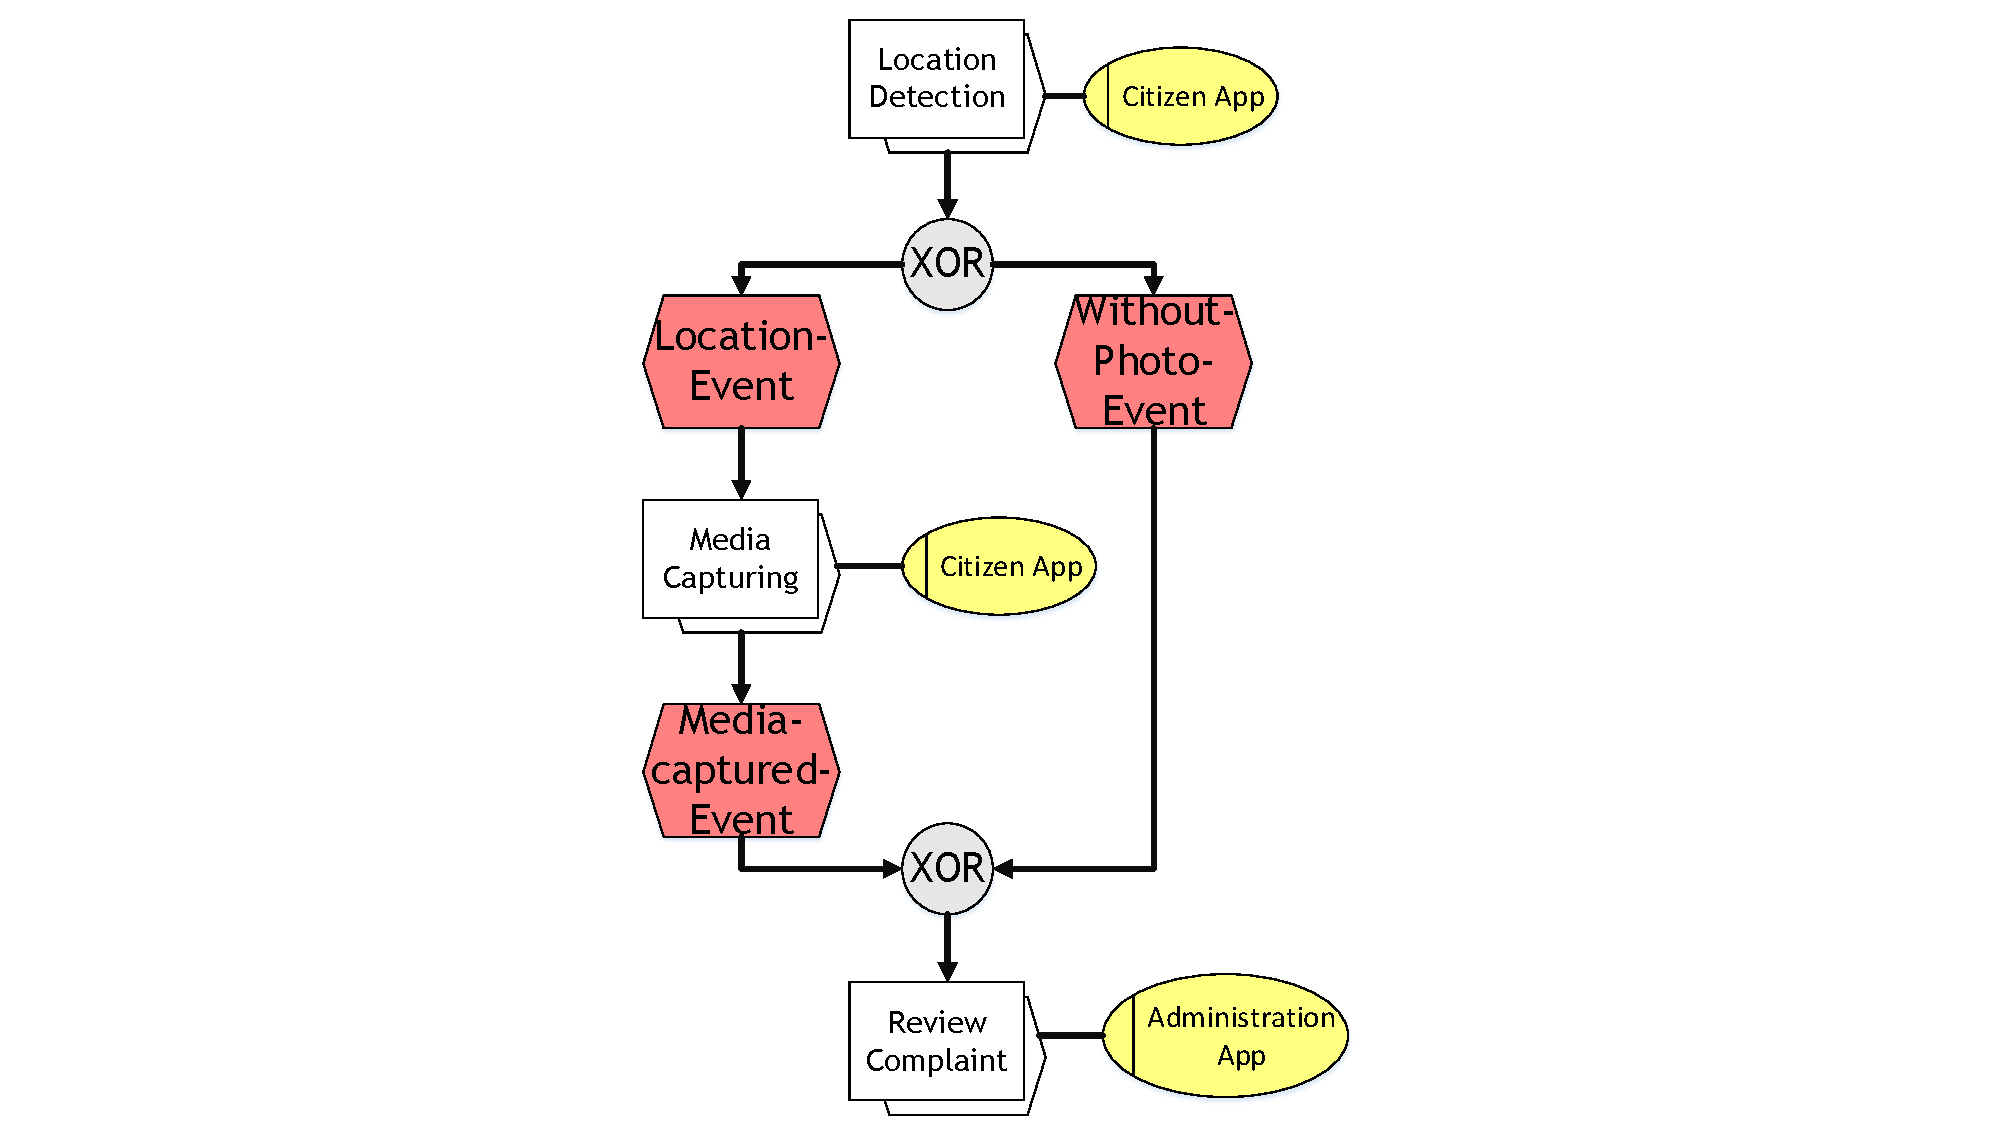
\includegraphics[height = 7cm, trim = 10cm 0cm 10cm 0cm, clip = true]{images/wfAcrossApps}	  
	\end{minipage}\hfill
	\begin{minipage}{0.5\textwidth}
\begin{lstlisting}
App CitizenApp {
  WorkflowElements {
    LocationDetection (startable: "Start Complaint"),
    MediaCapturing
  }
}

App AdministrationApp {
  WorkflowElements {
    ReviewComplaint
  }
}
\end{lstlisting}
\end{minipage}

\end{frame}

%-----------------------------------------------------------------------------------

\begin{frame}[plain]

\plainnumber

\frametitle{Implementation: WorkflowEventHandler}

\begin{center}
	\begin{tikzpicture}[
	>=stealth,
	wfe/.style = {draw, circle, fill=black!15!white},
	eh/.style = {draw, minimum height = 3cm, minimum width = 3cm, fill=pantone315!30!white}
	]
		\node (citizen) {
\includegraphics[width=0.5cm]{images/stickfigure}};
		\node[below = 0cm of citizen] (citizenlbl) {\scriptsize Citizen};
		
		\node[wfe, below = of citizenlbl] (wfe1) {WFE1};
		\node[wfe, below = of wfe1] (wfe2) {WFE2};
		\node[eh, right = 2cm of wfe1.north east, anchor = north west] (eh) {Event Handler};
		\node[draw, minimum width = 2cm, minimum height = 1cm, right = 2cm of eh, fill=pantone369!20!white] (be) {Backend};
		
		\begin{pgfonlayer}{bg}
			\draw[fill=pantone396!10!white, draw=pantone396] ($ (wfe1.north west) + (-0.4, 0.4) $) rectangle  ($ (eh.south east) + (0.5, -0.5) $);
		\end{pgfonlayer}
		
		\draw[->, thick, visible=<1->] (citizenlbl) -- node[right] {\scriptsize{\texttt{start}}} (wfe1);
		\draw[->, thick, visible=<2->] (wfe1) -- node[above, sloped] {\scriptsize{\texttt{ID, event}}} (eh);
		\draw[->, thick, visible=<3->] (eh.west) -- node[above, sloped] {\scriptsize{\texttt{changeWFE}}} (wfe2.north east);
		\draw[->, thick, visible=<4->] (wfe2.east) -- node[below, sloped] {\scriptsize{\texttt{ID, event}}} (eh);
		\draw[->, thick, visible=<5->] (eh) -- node[above] {\scriptsize{\texttt{ID, event}}} (be);
		
		\visible<6->{
			\node[above right = 0.75cm and 1.5cm of citizenlbl] (admin) {
\includegraphics[width=0.5cm]{images/stickfigure}};
			\node[below = 0cm of admin] (adminlbl) {\scriptsize Admin};
			\node[draw, fill=black!15!white, right = of admin, minimum width = 2cm, minimum height = 1cm] (looi) {LOOI};
			
			\draw[->, thick] (admin) -- node[above] {\scriptsize{\texttt{show}}} (looi);	
		}
		\visible<7>{
			\node[overlay, align=center,right = 0.5cm of looi, rectangle callout, drop shadow, fill=white, draw, minimum width = 2.5cm, minimum height = 1.5cm, callout absolute pointer = {(looi)}] (popup) {
				\begin{tikzpicture}
				{\tikzset{wtf/.style = {rectangle, draw=none, fill=none, minimum width = 0cm, minimum height = 0cm }}
					\draw (0,0) -- (2, 0);
					\draw (0.5, 0.25) -- ++(0, -1.25);
					\draw (1.25, 0.25) -- ++(0, -1.25);
					\node[wtf]  at (0, 0.15) {\tiny\texttt{ID}};
					\node[wtf] at (0.5, 0.15) {\tiny\texttt{WFE}};
					\node[wtf] at (1.25, 0.15) {\tiny\texttt{\dots}};
					\node[wtf] at (0, -0.3) {\tiny\texttt{01}};
					\node[wtf] at (0.5, -0.3) {\tiny\texttt{WFE1}};
					\node[wtf] at (1.25, -0.3) {\tiny\texttt{\dots}};
					\node[wtf] at (0, -0.6) {\tiny\texttt{02}};
					\node[wtf] at (0.5, -0.6) {\tiny\texttt{WFE3}};
					\node[wtf] at (1.25, -0.6) {\tiny\texttt{\dots}};
					\node[wtf] at (0, -0.9) {\tiny\texttt{03}};
					\node[wtf] at (0.5, -0.9) {\tiny\texttt{\dots}};
					\node[wtf] at (1.25, -0.9) {\tiny\texttt{\dots}};
					}
				\end{tikzpicture}
			};
		}
		\draw[->, thick, visible=<8->] ($(looi.east) + (0, 0.1) $) -| node[right] {\scriptsize{\texttt{appID}}} ($(be.north) + (0.1, 0)$);
		\draw[<-, thick, visible=<9->] ($(looi.east) + (0, -0.1) $) -| node[below left] {\scriptsize{\texttt{open issues}}} ($(be.north) + (-0.1, 0)$);
		\visible<10->{
			\node[wfe, below right = 0.5cm of looi] (wfe3) {WFE3};
			\draw[->, thick] (looi) |- node[above right] {\scriptsize{\texttt{start}}} (wfe3);	
		}
		\begin{pgfonlayer}{bg}
			\draw[fill=pantone396!10!white, draw=pantone396, visible=<6->] ($ (looi.north west) + (-0.4, 0.4) $) rectangle  ($ (wfe3.south east) + (0.5, -0.5) $);
		\end{pgfonlayer}		
	\end{tikzpicture}
\end{center}

\end{frame}

%-----------------------------------------------------------------------------------

\begin{frame}
    \frametitle{map.apps Architecture}
	\begin{center}
	\begin{tikzpicture}[
		>=stealth,
		box/.style = {draw, minimum width = 3cm, minimum height = 1.5em, outer sep=0},
		box2/.style = {box, minimum width = 3.5cm},
		node distance = 0.1cm
		]
		
		\node[box, fill=pantone315!10!white] (wfe1) {WfE 1};
		\node[box, right = of wfe1, fill=pantone315!10!white] (wfe2) {WfE 2};
		\node[box, minimum width=6.1cm, below = of wfe1.south west, anchor = north west, fill=pantone315!10!white] (wfEventHandler1) {WorkflowEventHandler};
		\node[box, below = of wfEventHandler1.south west, anchor=north west, fill=pantone315!10!white] (models1) {Models};
		\node[box, right = of models1, fill=pantone315!10!white] (contentProv1) {ContentProvider};
		\draw ($(wfe1.north west) + (-0.1, 0.6)$) node[below right] {\textbf{App 1}} rectangle ($(contentProv1.south east) + (0.1, -0.1)$);
		
		\node[box, below = 2.3cm of wfe1, fill=pantone315!10!white] (wfe3) {WfE 3};
		\node[box, below = 2.3cm of wfe2, fill=pantone315!10!white] (wfe4) {WfE 4};
		\node[box, below = of wfe3.south west, anchor = north west, minimum width=6.1cm, fill=pantone315!10!white] (wfEventHandler2) {WorkflowEventHandler};
		\node[box, below = of wfEventHandler2.south west, anchor=north west, fill=pantone315!10!white] (models2) {Models};
		\node[box, right = of models2, fill=pantone315!10!white] (contentProv2) {ContentProvider};
		\draw ($(wfe3.north west) + (-0.1, 0.6)$) node[below right] {\textbf{App 2}} rectangle ($(contentProv2.south east) + (0.1, -0.1)$);
		
		\draw[<->, thick] ($ (wfEventHandler1.east) + (0.1, 0) $) -- ++(0.8,0);
		\draw[<->, thick] ($ (wfEventHandler2.east) + (0.1, 0) $) -- ++(0.8,0);
		
		\node[box2, right = 1cm of wfe2.north east, anchor=north west, fill=pantone315!10!white]  (gb1) {List of open issues};
		\node[box2, below = of gb1, fill=pantone315!10!white] (gb2) {Runtime};
		\node[box2, below = of gb2, fill=pantone315!10!white] (gb3) {Location Service};
		\node[box2, below = of gb3, fill=pantone315!10!white] (gb4) {Workflow Store};
		\node[box2, below = of gb4, fill=pantone315!10!white] (gb5) {Local Store};
		\node[box2, below = of gb5, fill=pantone315!10!white] (gb6) {Store};
		\node[box2, below = of gb6, fill=pantone315!10!white] (gb7) {Formcontrols};
		
		\draw ($(gb1.north west) + (-0.1, 0.6)$) node[below right] {\textbf{Generic bundles}} rectangle ($(gb7.south east) + (0.1, -0.1)$);

		
		%\node[box, fill=pantone315!10!white] (model) {Model};
		%\node[box, below = of model] (dsl) {Domain-Specific\\Language};
		%\draw[<-] (model) -- node[right] (uses) {} (dsl);
		%\node[box, right = 1.75cm of uses] (generator) {Generator};
		%\node[box, right = of generator] (platforms) {Code for\\Platforms};
		%\draw[->] (dsl) -| (generator);
		%\draw[->] (model) -| (generator);
		%\draw[->] (generator) -- (platforms);
	\end{tikzpicture}
	\end{center}
\end{frame}

%-----------------------------------------------------------------------------------

\begin{frame}[fragile]
	\frametitle{Calling External Webservices}
	\begin{center}
	\begin{tikzpicture}[>=stealth,
		box/.style={minimum width = 2cm, minimum height = 1cm}]
		\node[box, fill=pantone396!10!white, draw=pantone396] (mapapps) {\mapapps\vphantom{Aq}};
		\node[box, right = 2cm of mapapps, fill=pantone369!20!white, draw=pantone369] (be) {Backend\vphantom{Aq}};
		\node[box, right = 2cm of be, fill=pantone315!20!white, draw=pantone315, align=center] (ws) {External\\Webservice\vphantom{Aq}};
		\draw[thick, transform canvas = {yshift=0.25cm}, ->] (mapapps) -- node[above] {\footnotesize\texttt{JSON data\vphantom{Aq}}} (be);
		\draw[thick, transform canvas = {yshift=-0.25cm}, <-] (mapapps) -- node[below] {\footnotesize\texttt{{\color{pantone390!80!black}200}/\alert{404}\vphantom{Aq}}} (be);
		\draw[thick, transform canvas = {yshift=0.25cm}, ->] (be) -- node[above] {\footnotesize\texttt{request\vphantom{Aq}}} (ws);
		\draw[thick, transform canvas = {yshift=-0.25cm}, <-] (be) -- node[below] {\footnotesize\texttt{response\vphantom{Aq}}} (ws);
	\end{tikzpicture}
	\end{center}
	
	\vfill
	
	\begin{itemize}
		\item Backend acts as a proxy for all webservice calls
		\item Transforms JSON-encoded object into request
		\item (Currently) only returns status code for success or failure
	\end{itemize}
\end{frame}

%-----------------------------------------------------------------------------------

\begin{frame}[fragile]
	\frametitle{Calling External Webservices}
\begin{lstlisting}[basicstyle=\footnotesize\ttfamily]
externalWebService sendEmail {
   url "http://psmd2.uni-muenster.de:8080/SendMail/api/mail/send/"
   method GET
   queryparams (
     "to" : "md2@trashmail.de"
     "subject" : "Map.Apps E-Mail"
     "body" : "Dear ladies and gentlemen, this is an e-mail sent by md2 map.apps!"
   )
}
\end{lstlisting}
\codeheading{Usage within a Workflow Element}
\begin{lstlisting}[basicstyle=\footnotesize\ttfamily]	
bind action WebServiceCall sendEmail on myView.myBtn.onClick
\end{lstlisting}
\end{frame}

%-----------------------------------------------------------------------------------

\begin{frame}
\frametitle{Starting Workflows from External WS Calls}

\begin{tikzpicture}[
	>=stealth,
	block/.style = {draw, fill=white, minimum width = 4cm,  minimum height = 1.75em}]
	\node[draw=pantone315, minimum width = 4cm, fill=pantone315!30!white, align=center] (IS) {External\\Information System};
	\node[block, below = 1.5cm of IS] (WS) {WS to start WFE1};
	\node[block, below = of WS] (wfe1) {WorkflowState WFE1};
	\node<2->[block, right = 1.5cm of WS] (looi) {List of open issues};
	
	\begin{pgfonlayer}{bg}
		\draw[fill=pantone369!20!white, draw=pantone369] ($ (WS.north west) + (-0.5, 0.5) $) node[above right] {\scriptsize\color{gray}Backend\vphantom{Aq}} rectangle ($ (wfe1.south east) + (0.5, -0.5) $);
		\draw<2->[fill=pantone396!20!white, draw=pantone396] ($ (looi.north west) + (-0.5, 0.5) $) node[above right] {\scriptsize\color{gray}\mapapps app\vphantom{Aq}} rectangle ($ (looi.south east) + (0.5, -0.5) $) ;
	\end{pgfonlayer}
	
	\draw[->] (IS) -- node[above right] {\texttt{\scriptsize{call}}} (WS);
	\draw[->, transform canvas = {xshift=-1.5cm}] (WS) -- node[right] {\texttt{\scriptsize{create}}} (wfe1);
	\draw<2->[->] (looi) |- node[above left] {\texttt{\scriptsize{load}}} (wfe1);
\end{tikzpicture}

\end{frame}

%-----------------------------------------------------------------------------------

\begin{frame}[fragile]
	\frametitle{Starting Workflows from External WS Calls}
\codeheading{Workflow Layer}
\begin{lstlisting}[basicstyle=\footnotesize\ttfamily]
WorkflowElement LocationDetection (invokable)
  fires ...
\end{lstlisting}
\codeheading{Controller Layer}
\begin{lstlisting}[basicstyle=\footnotesize\ttfamily]		
invokable at "address" using POST {
  set :ComplaintProvider.loc to :AddressProvider
  :AddressProvider.myStreet
  :AddressProvider.myStreetNo
  :AddressProvider.myCity
  :AddressProvider.myPostalCode
  default :ComplaintProvider.status = "User is filling out complaint" 
}
\end{lstlisting}
\end{frame}

%-----------------------------------------------------------------------------------

\begin{frame}[fragile]
\frametitle{Location Action}

\begin{itemize}
\item Calculates coordinates from a given address and stores them
\item Uses the ArcGIS API for JavaScript
\end{itemize}

\begin{lstlisting}[basicstyle=\footnotesize\ttfamily]
action Location (
    inputs (
       cityInput :AddressProvider.myCity
       streetInput :AddressProvider.myStreet
       streetNumberInput :AddressProvider.myStreetNo
       postalInput :AddressProvider.myPostalCode
       countryInput :AddressProvider.myCountry
    )
    outputs (
       latitudeOutput :AddressProvider.myLatitude
       longitudeOutput  :AddressProvider.myLongitude
    ))		 				
\end{lstlisting}

\end{frame}

%-----------------------------------------------------------------------------------

\begin{frame}[plain]
\frametitle{Upload Images}
\plainnumber
\begin{center}
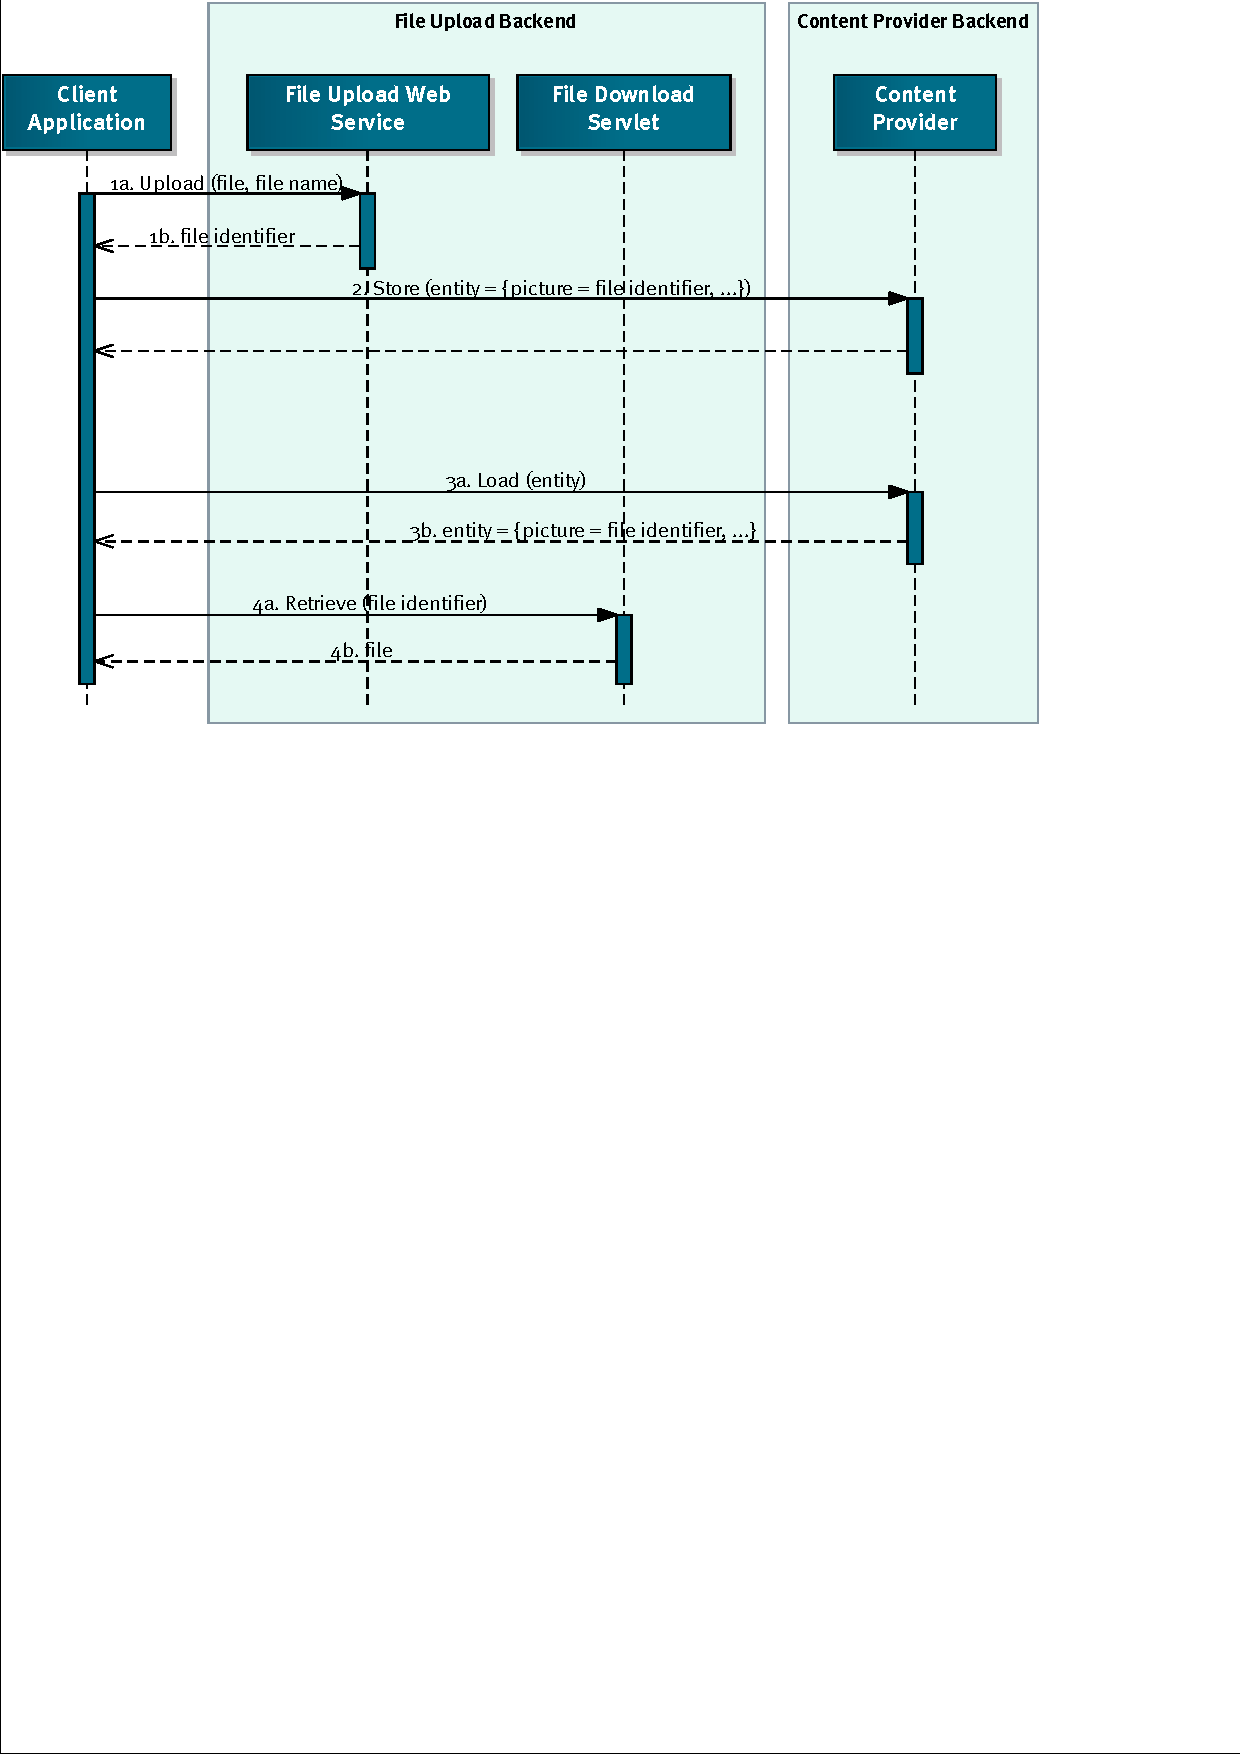
\includegraphics[width=1\textwidth, trim = 0.5mm 10cm 3.3cm 0.5mm, clip = true] {images/UML-diagrams.pdf}
\end{center}
\end{frame}

\begin{frame}[fragile]
\frametitle{Upload Images}
\codeheading{View Layer}
\begin{lstlisting}[basicstyle=\footnotesize\ttfamily]
FileUpload UploadBtn {text "Upload File"}
UploadedImageOutput imageoutput
\end{lstlisting}

\vfill

\codeheading{Controller Layer}
\begin{lstlisting}[basicstyle=\footnotesize\ttfamily]
main {
	...  
	fileUploadConnection UploadConnection
}
map MediaCapturingView.UploadBtn to :ComplaintProvider.picture
map MediaCapturingView.imageoutput to :ComplaintProvider.picture
\end{lstlisting}
\end{frame}

%-----------------------------------------------------------------------------------

%\begin{frame}
%    \frametitle{Generator}
%    
%	\begin{center}   
%	\begin{tikzpicture}[
%		>=stealth,
%		node distance = 0.75cm and 0.25cm,
%		every node/.style={minimum height = 1.75em}]
%		\node[draw] (dsl) {DSL\vphantom{Aq}};
%		\node[draw, below = of dsl] (md2model) {\MD Model\vphantom{Aq}};
%		\draw[->] (md2model) -- node[right] {\tiny{uses}} (dsl);
%	    
%		\node[below = of md2model, draw] (preprocessor) {Preprocessor\vphantom{Aq}};
%		\draw[->] (md2model) -- node[right] {\tiny{processed by}} (preprocessor);
%		
%		\node[draw, below = of preprocessor] (generator) {Generator\vphantom{Aq}};
%		
%		\draw[->] (preprocessor) -- node[right] {\tiny{input for}} (generator);
%		
%		\node[draw, below left = 0.25cm of generator] (mapapps) {map.apps source\vphantom{Aq}};
%		\node[draw, below right = 0.25cm of generator] (backend) {backend source\vphantom{Aq}};
%		
%		\draw[->] (generator) -| node[above] {\tiny{generates}} (mapapps);
%		\draw[->] (generator) -| node[above] {\tiny{generates}} (backend);
%	\end{tikzpicture}
%	\end{center}
%\end{frame}

%\begin{frame}
%    \frametitle{Deployment}
%    
%    \begin{center}   
%	    \begin{tikzpicture}[
%	    >=stealth,
%	    node distance = 0.75cm and 0.25cm,
%	    big/.style = {draw, minimum width = 2.5cm, minimum height = 1.75em}
%	    ]
%	    \node[big] (generator) {Generator};
%	    \node[big, below left = of generator] (mapapps) {map.apps source\vphantom{Aq}};
%	    \node[big, below right = of generator] (backend) {backend source\vphantom{Aq}};
%	    \draw[->] (generator) -| node[above] {\tiny{generates}} (mapapps);
%	    \draw[->] (generator) -| node[above] {\tiny{generates}} (backend);
%	    \node[big, rounded corners, below = of mapapps] (jetty) {Jetty\vphantom{Aq}};
%	    \node[big, rounded corners, below = of backend] (glassfish) {Glassfish\vphantom{Aq}};
%	    \draw[->] (mapapps) -- node[left] {\tiny{deployed on}} (jetty);
%	    \draw[->] (backend) -- node[right] {\tiny{deployed on}} (glassfish);
%	    \draw[<->] (jetty) -- node[above] (communicates) {\tiny{communicates}} (glassfish);
%	    
%	    \node[big, rounded corners, below = of communicates] (tomcat) {Tomcat};
%	    \node[big, gray, below = 0cm of tomcat] {map.apps full};	    
%	    
%	    \end{tikzpicture}
%    \end{center}
%\end{frame}

%-----------------------------------------------------------------------------------

\begin{frame}
    \frametitle{Modeling, Generation \& Deployment}
    
    \begin{center}   
	    \begin{tikzpicture}[
	    >=stealth,
	    node distance = 0.75cm and 0.25cm,
	    big/.style = {draw, minimum width = 2.5cm, minimum height = 1.75em},
	    header/.style = {big, minimum width = 3.2cm, fill=pantone315!10!white, outer sep = 0}
	    ]
	    \node[header] (eclipseDevelopment) {Framework IDE};
	    \node[big, below = 0.05cm of eclipseDevelopment] (dsl) {DSL};
	    \node[big, below = 0.05cm of dsl] (generator) {Generator};
	    
	    \node[below=1.4cm of generator, header] (generatedArtifacts) {Generated Artifacts\vphantom{Aq}};
	    \node[big, below = 0.05cm of generatedArtifacts] (backend) {Backend};
	    \node[big, below = 0.05cm of backend] (mapApps) {map.apps};
	    
	    \node[big, right = 2cm of backend, fill=pantone315!10!white] (glassfish) {Glassfish AS};
	    \node[big, right = 2cm of mapApps, fill=pantone315!10!white] (jetty) {Jetty};
	    
	    \draw[->] (backend) -- node[above] {\tiny{deploy}} (glassfish);
	    \draw[->] (mapApps) -- node[above] {\tiny{deploy}} (jetty);
	    
	    \node[header, right = 2cm of eclipseDevelopment] (eclipseModeling) {Modeling IDE};
	    \node[big, below = 0.05cm of eclipseModeling] (md2model) {\MD Model};
	    \node[below = 0cm of md2model] (modelModels) {models};
	    \node[below = 0cm of modelModels] (modelViews) {views};
	    \node[below = 0cm of modelViews] (modelController) {controllers};
	    \node[below = 0cm of modelController] (modelViews) {workflows};
	    
	    \draw[->] (md2model) -- node[above] {\tiny{uses}} (dsl);
	    \draw[->] (generator) -- node[left] {\tiny{generates}} (generatedArtifacts);
	    \draw[->] ($(eclipseModeling.south west) + (0, -1.125)$) -- node[above] {\tiny{invokes}} (generator);   

	    \draw (eclipseDevelopment.north west) rectangle ($(eclipseDevelopment.south east) + (0, -1.7)$);
	    \draw (generatedArtifacts.north west) rectangle ($(generatedArtifacts.south east) + (0, -1.7)$);
	    \draw (eclipseModeling.north west) rectangle ($(eclipseModeling.south east) + (0, -3.5)$);
	    \draw (md2model.south west) rectangle ($(md2model.south east) + (0, -2.5)$);
	    
	    
	    \end{tikzpicture}
    \end{center}
\end{frame}
